\chapter{Review of related software libraries}
\label{chapt:technology}
In this chapter, we introduce libraries that can be beneficial for creating a destructible environment. We do not talk about all-in-one software development kits with their approach to a destructible environment already implemented. Instead, our focus is on building a game with the destructible environment from zero.  

To build a game we will surely need a physics engine, a graphics engine, and to support our destructible environment a selection of geometric libraries. We mention which libraries we used in the implementation and details of their use can be found in~\cref{app:implementation}.

We committed ourselves to writing our application in \emph{C++} language and using only free software. This commitment limits us in the availability of certain software. 

\section{Physics engine}
Bullet Physics
\todo {text here}


\section{Rendering engine}
Rendering engine creates a base for a computer game. It allows a player to see the current state of the game world and control the game. Today, two most common libraries providing API for communication with GPU are \emph{OpelnGL} and \emph{DirectX}. Although it is possible directly use those low-level libraries, we use a library with more abstraction in provided API. Using higher-level libraries means we can save code, but we lose a direct control of rendering process. This thesis is not focused on graphical output and only uses it as a tool for building our application.

We decided to use \textbf{Irrlicht Engine}~\footnote{http://irrlicht.sourceforge.net/}. Irrlicht is a light-weight cross-platform, high-performance engine capable of using either  \emph{OpelnGL} or \emph{DirectX}. Our use of Irrlicht is based on using its graphical window as an output of our application and also using Irrlichts event receiver for reading user input.

\section{Geometric libraries}
Here we introduce a set of libraries focused on a decomposition or modification of 3D meshed objects. We categorise them by provided function.

\subsection{Boolean operations}
When searching for efficient library able to compute the difference of two 3D triangular meshes, we found out that the majority of available software is dependent on using \textbf{The Computational Geometry Algorithms Library}~\footnote{http://www.cgal.org/} or shortly \textbf{CGAL}. CGAL provides polyhedral surfaces that are closed for Boolean operations, and it is possible to convert data between meshes and polyhedrons. The choice to use CGAL creates restrictions on 3D meshes we can use (for more details on data structure see~\cref{app:implementation}).

We considered using a \textbf{Cork Boolean Library}~\footnote{https://github.com/gilbo/cork\#cork-boolean-library} but we did not find it to be as robust as CGAL.

\subsection{Voronoi tessellation}
We learned that to Voronoi tessellation can be beneficial to either creating a compound body held together by springs or used as a tool for subtracting parts of the mesh. Here are some libraries useful for both tasks.

\begin{description}
\item[CGAL] also includes package providing different 3D triangulations, mainly Delaunay triangulation and the possibility of creating Voronoi diagram as its dual graph. However, CGAL does not provide means to clip the Voronoi cells against the surface mesh.

\item[Voro++]\footnote{http://math.lbl.gov/voro++/} is a library for carrying out three-dimensional computations of the Voronoi tessellation. It calculates Voronoi cell for each particle individually and is suited for high-performance calculations on large scale particle systems. It is also able to clip Voronoi cells to any user defined boundary. This library would be well suited for decomposing entire objects into Voronoi cells. 

Because implementation requires only one Voronoi cell per collision, we chose to use the simpler Voro++ library for this task. 
\end{description}


\subsection{Convex decomposition}
\label{sec:decompositionLib}
Convex decomposition is critical to fast and accurate collision detection on 3D meshes. We introduce two libraries with different approaches to the task.
\begin{description}
\item[CGAL] provides the means for decomposing the polyhedral shape (triangular mesh can be converted into polyhedron) into a set of convex polyhedrons. CGAL is aiming for an exact convex decomposition, which produces a large number of small pieces~\footnote{http://doc.cgal.org/latest/Convex\_decomposition\_3}.

\item[Hierarchical Approximate Convex Decomposition] or HADC~\cite{HACD} is a library and algorithm providing a convex decomposition that approximates the original shape. The approximation yields fewer pieces and is faster than exact calculations, but the result is not exact. For the reasons that we are implementing a destructible environment in a computer game, we can allow for deviations in the shape of the objects from their respective visual representations. Those deviations should be too small to be noticed in the game. This makes us choose HACD over CGAL.
\end{description}

We can see the difference in the result of those two approaches on~\cref{fig:bunny}. It is evident that we do not want to use the exact decomposition in a computer game, but on the other hand for the simulations where the calculation time is not critical, the approximations should not be used.
\begin{figure}
        \centering
        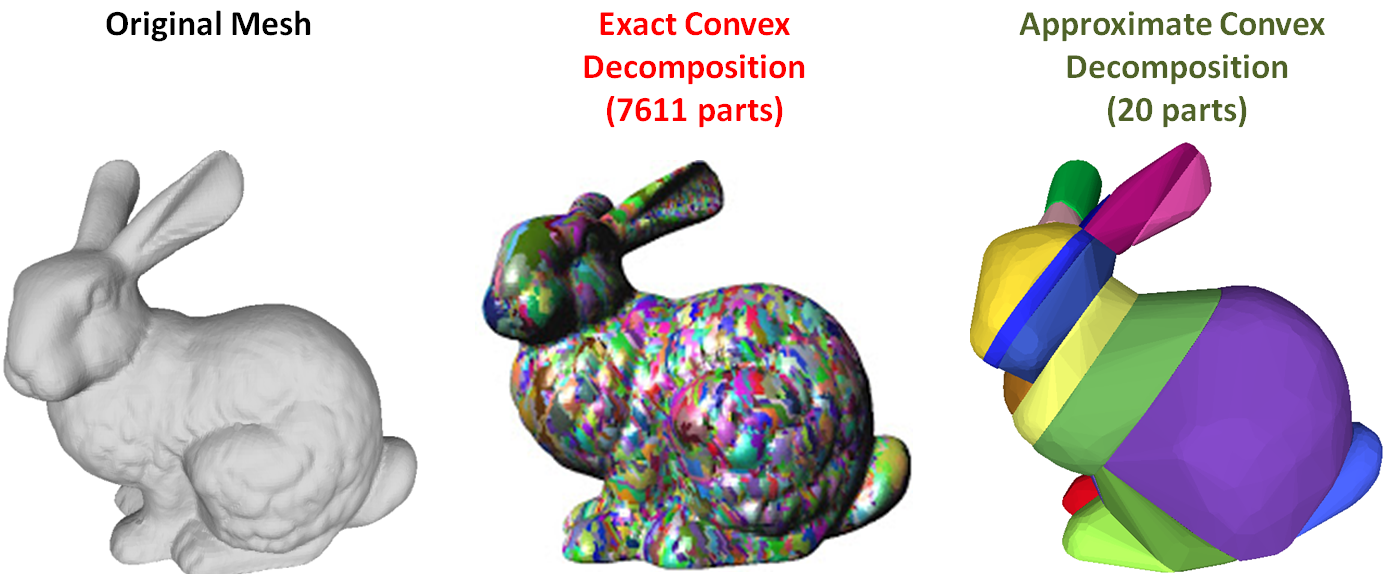
\includegraphics[width=\textwidth]{img/bunny}
        \caption{Difference between original mesh, exact convex decomposition and an approximate convex decomposition. Source: https://github.com/kmammou/v-hacd}
        \label{fig:bunny}
\end{figure}


